\subsection{Differential Forms}
The next step of course is to determine how we integrate on complex manifolds. As usual, we integrate forms. A holomorphic differential (1-)form $\omega$ on a complex manifold $M$ assigns a covector of the tangent space to every point on the manifold in a holomorphic manner. Another way to say this is that when viewed through coordinate charts $\omega$ is a holomorphic differential form on an open subset of $\C$ (as we have dealt with earlier). 

To be precise suppose $(\varphi_i, U_i)$ is a coordinate charts on $M$. Then we get a differential form $\omega_i$ on $\varphi_i(U_i)$ by pushing forward $\omega$ (we can do this because $\varphi_i$ is a biholomorphism onto its image). Since $\omega_i$ is a differential form on an open subset of $\C$ we know it is of the form $\omega_i = f_i(z) dz$ where $f_i$ is a holomorphic map. 

Now suppose $(\varphi_j, U_j)$ is another coordinate chart where we denote the coordinates by $w$ (which is to say $w = \varphi_j(x)$ for $x \in U_j$). Then as before we get a differential form on $\varphi_j(U_j)$, which we denote $\omega_j = f_j(w) dw$. We of course want the two forms to agree on the overlap, $\varphi_i(U_i \cap U_j)$. What does it mean to agree on the overlap? Let $g_{ij}$ be the biholomorphism from $\varphi_i(U_i \cap U_j)$ to $\varphi_j(U_i \cap U_j)$ so that $w = g_{ij}(z)$. Therefore we have 
\begin{align*}
    \omega_j = f_j(w)dw = f_j(g_{ij}(z)) d(g_{ij}(z)) = f_{j}(g_{ij}(z)) g'_{ij}(z) dz
\end{align*} 
Then to say that the forms agree on the overlap we must have 
\begin{align*}
    f_{j}(g_{ij}(z)) g'_{ij}(z) dz = f_i(z) dz
\end{align*}

As before if $\omega$ is a holomorphic differential form on a complex manifold $M$, then by Cauchy's Theorem we know that a holomorphic differential form $\omega$ is closed and therefore has a local primitive. This means for every point, there exists a neighbourhood of it such that there is a holomorphic function $g$ defined on this neighbourhood such that $\omega = dg$. In general, $\omega$ will not have a global primitive. As before, a differential form has a global primitive (i.e. is exact) if and only if 
$$\int_\gamma \omega = 0$$
for every closed curve $\gamma$. In particular this means that every holomorphic differential form on a simply connected complex manifold has a global primitive. Even if the integral of $\omega$ over closed curves is not zero, it provides important information about the form and the geometry of the surface. We call the integral of $\omega$ over closed curves the periods of $\omega$.

\secbreak

One of the most important tools for evaluating complex integrals is the Residue Theorem. The theorem still holds on general complex manifolds and hence serves as a very powerful tool for studying the geometry of these surfaces. 

Suppose $\omega$ is a holomorphic differential form defined on the complement on a discrete set $E \subset M$ and let $a \in E$. Recall that the residue of $\omega$ at $a$ is then defined to be
$$Res(\omega, a) = \frac{1}{2\pi i} \int_\gamma \omega$$
where $\gamma$ is a simple closed curve with winding number 1 (with respect to $a$). We can compute it using local coordinates. Let $z$ be local coordinates at $a$ and we can assume that $z(a) = 0$. Then 
\begin{align*}
    \omega = \left( f(z) + \frac{c_1}{z} + \frac{c_2}{z^2} + \cdots \right) dz
\end{align*}
where $f$ is holomorphic near $a$. Then we compute that the residue of $\omega$ at $a$ is $c_1$. With our understanding of residues, the Residue Theorem exactly as it did before.
\begin{theorem}[Residue Theorem]
    Let $\Omega$ be an open subset of a complex manifold $M$ and $f(z)$ a holomorphic function on the complement of a discrete set in $\Omega$. Let $K$ be a compact subset of $\Omega$ with piecewise $C^1$ boundary $\Gamma$. Then
    $$\int_{\Gamma} f(z) dz = 2\pi i \sum_{z_k \in K} \text{Res}(f, z_k)$$
    where $S$ is the set of singular points of $f$ in $K$. 
\end{theorem}

\subsection{Riemann Surfaces}
Let $Y$ be a complex curve (most often $\C, S^2$ or an open subset of these). Then a Riemann surface over $Y$ is a connected complex curve $X$ along with a nonconstant holomorphic map $\varphi: X \to Y$. 

A branch point of $\varphi$ (or of $X$) is a point where $\varphi$ has multiplicity greater than 1 (equivalently where $\varphi'$ is 0). Branch points are isolated and the preimage of any point of $Y$ is discrete (both statement follow form the fact that zeroes of a non-zero holomorphic function are isolated). A Riemann surface without branch points is called unramified. Importantly, $\varphi$ need not be injective even if the the surface is unramified. 

\begin{example}
    A simple example to start with is to take $Y = \C \setminus \{0\}$ and $X = \C$ with $\varphi: X \to Y$ given by $\varphi(z) = e^z$. 

    In this case not only is $X$ a Riemann surface over $Y$, it in fact forms a \textit{covering space} of $Y$. This means that $X$ is an unramified surface and every point of $Y$ has an open neighbourhood $V$ such that $\varphi^{-1}(V)$ is a disjoint union of open sets $U_i$ where each $U_i$ is mapped homeomorphically to $V$ via $\varphi$. In this case with $X, Y, \varphi$ as above, for $b \in Y = \C \setminus \{0\}$ we can take $V = \{\abs{z - b} < \abs{b}\}$. 

    % TODO: Add diagram
\end{example}
\begin{figure}[ht]
    \centering
    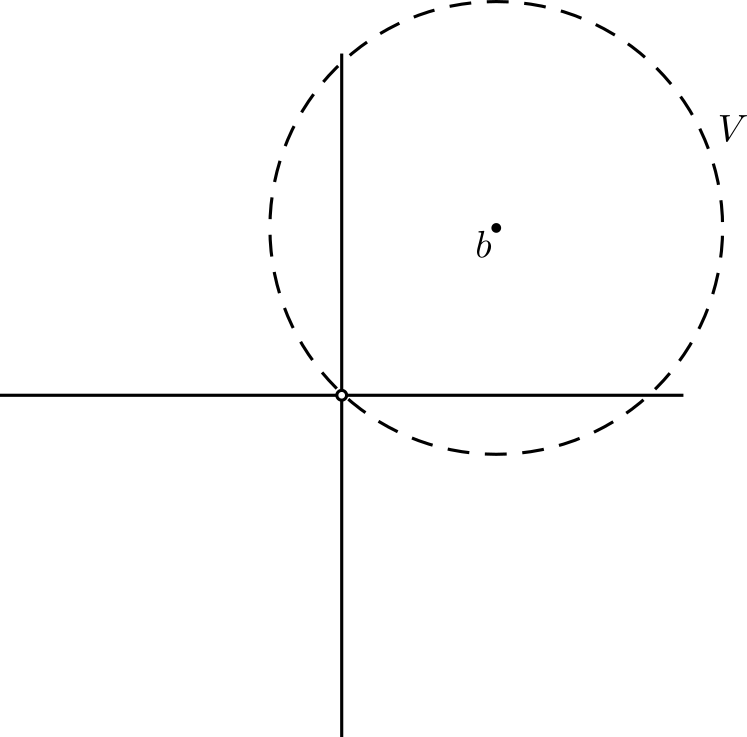
\includegraphics[scale=0.5]{Images/log_cover_riem_surf.png}
    \caption{$\log$ has a holomorphic branch on $V$ serving as a coordinate map}
    \label{fig:log-cover-riem-surf}
\end{figure}

\begin{example}
    A very important use of Riemann surfaces is to make multi-valued functions single-valued. Consider for example the square root function $y = x^{1/2}$. In order to make this single-valued, consider 
    $$X := \{(x, y) \in \C \times \C | x = y^2\}$$ 
    This forms a Riemann surface over $Y = \C$ with $\varphi: X \to \C$ given by $\varphi(x, y) = x$. Then the square root function $Y \to \C$ given by $z \mapsto \sqrt{z}$ lifts to the map $p(x, y) = y$ from $X$ to $\C$. 

    \adjustbox{scale=1.1, center}{
        % https://tikzcd.yichuanshen.de/#N4Igdg9gJgpgziAXAbVABwnAlgFyxMJZABgBoAmAXVJADcBDAGwFcYkQAPAAgB0ewsXAJogAvqXSZc+QijLFqdJq3YAKDqS4BPAJS9+ggBp80AC3pgcEALbB69LKLESQGbHgJEAjKS+KGLGyIIHzW9DimAEaRwADCTqKKMFAA5vBEoABmAE42SD4gVkjkNIxYYEEgUPRwpskgpfSRMIwAClIesiCMMJk4DUqB7GjOWbnWSGSFEMU0ASrBfHAAjtk4wABeTo3NbR0y7NlYKab94mN5iAVFiFO1WH1IALTk5yA5l9cztzT3j4glQoORjsMJoOBFRKiIA
        \begin{tikzcd}
            {(x, y) \ni X\phantom{aai}} \arrow[rd, "p", dashed] \arrow[dd, shift left=2] \arrow[dd, maps to, shift right=2] &            \\
                                                                                                                            & \mathbb{C} \\
            x \ni Y \arrow[ru, "\sqrt{z}"']                                                                                 &           
        \end{tikzcd}
    }
    % TODO: diagram
\end{example}

\subsection{Worked Example}
\subsubsection{Manifold construction}
Consider the multivalued function
$$y = (1 - x^3)^{1/3}$$
We want to find a Riemann surface so that this function is single-valued over it. As we did with $\sqrt{z}$ we take 
\begin{align*}
    X := \{(x, y) \in \C \times \C : x^3 + y^3 = 1\}
\end{align*}
We first show that $X$ is a manifold. Consider the function
$$f(x, y) = x^3 + y^3$$
Notice that 
\begin{align*}
    \frac{\partial f}{\partial y}(x_0, y_0) = 3y_0^2
\end{align*}
Therefore if $y_0 \neq 0$ then $\frac{\partial f}{\partial y} (x_0, y_0) \neq 0$ so by the Implicit Function Theorem (see \autoref{thm:weak-imft}), we can express $y$ as a function of $x$ implying that $x$ serves as a coordinate in this region. In particular, near $(x_0, y_0)$ $X$ is given as the graph of the function $x \mapsto \sqrt[3]{1 - x^3}$ with a choice of branch which is equal to $y_0$ when $x = x_0$. Hence, to be precise, for every $(x_0, y_0) \in X$ where $y_0 \neq 0$, we have that the projection onto the first coordinate $x$ (along with a choice of choice of cube root) serves locally as a coordinate chart. Similarly if $x_0 \neq 0$ then $y$ (i.e. projection onto the second coordinate) serves as a local coordinate on $X$. 

We want to check that the transition maps, when $x_0 \neq 0$ and $y_0 \neq 0$, are holomorphic. The first coordinate chart $\varphi_1$ is given by $(x, \sqrt[3]{1 - x^3}) = (x, y) \mapsto x$ and the second chart $\varphi_2$ by $(\sqrt[3]{1 - y^3}, y) = (x, y) \mapsto y$. Then 
\begin{align*}
    (\varphi_1 \circ \varphi_2^{-1})(y) = \sqrt[3]{1 - y^3}
\end{align*}
which is holomorphic since we chose a holomorphic branch of $\sqrt[3]{1 - y^3}$ (to be specific we chose a branch so that $x_0 = \sqrt[3]{1 - y_0^3}$). The analogous argument holds for $\varphi_2 \circ \varphi_1^{-1}$. Therefore $X$ is indeed a manifold.

Now we want to consider the original function $y = \sqrt[3]{1 - x^3}$ and its lift to $X$. The commutative diagram is then the exact same as above

\adjustbox{scale=1.1, center}{
        % https://tikzcd.yichuanshen.de/#N4Igdg9gJgpgziAXAbVABwnAlgFyxMJZABgBoAmAXVJADcBDAGwFcYkQAPAAgB0ewsXAJogAvqXSZc+QijLFqdJq3YAKDqS4BPAJS9+ggBp80AC3pgcEALbB69LKLESQGbHgJEAjKS+KGLGyIIHzW9DimAEaRwADCTqKKMFAA5vBEoABmAE42SD4gVkjkNIxYYEEgUPRwpskgpfSRMIwAClIesiCMMJk4DUqB7GjOWbnWSGSFEMU0ASrBfHAAjtk4wABeTo3NbR0y7NlYKab94mN5iAVFiFO1WH1IALTk5yA5l9cztzT3j4glQoORjsMJoOBFRKiIA
        \begin{tikzcd}
            {(x, y) \ni X\phantom{aai}} \arrow[rd, "p", dashed] \arrow[dd, shift left=2] \arrow[dd, maps to, shift right=2] &            \\
                                                                                                                            & \mathbb{C} \\
            x \ni Y \arrow[ru, "{\sqrt[3]{1 - x^3}}"']                                                                                 &           
        \end{tikzcd}
    }
with $Y = \C$ and $p(x, y) = y$, as we had before.

In general, for a given $y$, there are 3 distinct points in $X$ such that $p(x, y) = y$. These correspond to the three choices of the cube root of course. However, these points coincide when $x$ is a cube root of unity since then we are taking the cube root of 0. Therefore $(1, 0), (j, 0)$ and $(j^2, 0)$, where $j = e^{2\pi i/3}$ are branch points of $X$ (although quite often we identify the branch points with their images in $Y$, so one might simply say that the branch points of the Riemann surface are $1, j$ and $j^2$). 

\subsubsection{Extension of Riemann Surface}
Currently $X$ is simply a Riemman surface over $\C$. One might wonder whether it extends to be a Riemann surface over $S^2$. This is analogous to how the real line is a smooth (real) curve in $\C$ but it can be compactified and extended to be a curve (and in fact a closed curve) in $S^2$.  

Therefore first we will need to compactify $X$ and find the `points at infinity'. Then we will verify whether these points can be mapped to $\infty \in S^2$ holomorphically.

We compactify the curve by considering it as a subset of $P^2(\C)$. Recall that we have 
$$P^2(\C) = \{[x, y, t]: t \neq 0\} \sqcup \{[x, y, t]: t \neq 0\} $$
The first set can be identified with $\C \times \C$ with the coordinate chart $[x, y, t] \mapsto (x/t, y/t)$. Then the line (notice line, not point) through infinity is exactly the second set, where $t = 0$.  With respect to the identification above, the equation of the curve $X$ is given by 
$$ \left(\frac{x}{t}\right)^3 + \left( \frac{y}{t} \right)^3 = 1 $$
which we can rearrange to 
$$x^3 + y^3 = t^3$$
This is exactly what it means to homogenise the equation. Let $X'$ be the points in $P^2(\C)$ that satisfy this equation (this is the compactification of $X$). The points at infinity are exactly when $t = 0$. Therefore they are given by $[x, y, 0]$ satisfying
$$x^3 + y^3 = 0$$
Of course the point $(0, 0, 0)$ is not an element of $P^2(\C)$ so in particular $y$ must be non-zero (in fact both $x$ and $y$ must be non-zero). Finally since $[x, y, 0] = [x/y, 1, 0]$, we can conclude that the 3 points at infinity are $[-1, 1, 0], [-j, 1, 0]$ and$[-j^2, 1, 0]$ where recall $j = e^{2\pi i/3}$. Therefore
$$X' = X \cup \{[-1, 1, 0], [-j, 1, 0], [-j^2, 1, 0]\}$$

Let $\varphi': X' \to S^2$ be an extension of $\varphi: X \to \C$ so that it agrees with $\varphi$ on $X$ and maps the 3 points at infinity to $\infty \in S^2$. We want to check whether not $\varphi$ is holomorphic. We already know this is the case for points away from the points at infinity so we only need to check at those three points. 

Notice that at the three points at $\infty$ $y$ is never 0. Therefore we can verify holomorphicity in this chart. In this chart the curve is given by dehomogenising with respect to $y$ so that we are looking at 
$$x'^3 - t'^3 + 1 = 0$$
where $x' = x/y$ and $t' = t/y$. Since the partial derivative of the left hand side with respect to $x$ is non-zero at $(-j^k, 0)$ for $k = 0, 1, 2$ we conclude that $t'$ acts as a local coordinate with $x' = \sqrt[3]{1 - (t')^3}$. Then we compute what this map looks like at the level of coordinate charts.

\adjustbox{scale=1.1, center}{
    % https://tikzcd.yichuanshen.de/#N4Igdg9gJgpgziAXAbVABwnAlgFyxMJZABgBpiBdUkANwEMAbAVxiRAFUQBfU9TXfIRQBGclVqMWbABoBybrxAZseAkQBMY6vWatEIAMoA9dQAIAOubgwcAWyxgmcC+eAHLXBXxWCiAZi0JXTZLWzocAAsAIyjgAGFPHm8BNRQyYXEdKX0ceSSlflUhZFEM7Uk9EGRLOABHACccZD8KYGFTAFpTAApcgEojPx5TUVNcii8Cn1TkTTKg7JBLenq0CKxu6vMAM3q6AGNgGoamlrbOnv7Bri5gXOHLXYO22-vSEYpTPsnlFOKA+ZZSqPPaHe5HKwnZqtdpdXqyAZDRLiGBQADm8CIoF2EFsSDIIBwECQwnyOLxiFEhOJiHUZPquKQmmpSCGinJSAALNQiUgAKw8uhYBhsMJoOC8+mMxAClmIABsguForo4sl7IZFMVcoA7EqRfoxRLiVwKFwgA
    \begin{tikzcd}
        \C \setminus \{0\} \supset U \arrow[r]           & X' \arrow[r]                                       & S^2 \setminus \{S\} \arrow[r]                                                     & \mathbb{C}                        \\
        t' \arrow[r, maps to] & {[\sqrt[3]{1 - (t')^3}, 1, t']} \arrow[r, maps to] & {\varphi([\frac{\sqrt[3]{1 - (t')^3}}{t'}, \frac{1}{t'}, 1] )} \arrow[r, maps to] & {\frac{t'}{\sqrt[3]{1 - (t')^3}}}
    \end{tikzcd}
}
where for the final mapping we use the coordinates at infinity in $S^2$ (so although as a map into $\C$ we had $\varphi([x, y, 1]) = x$, when we switch to the coordinates at $\infty$ this becomes $[x, y, 1] \mapsto 1/x$). Therefore overall the map is given by 
\begin{align*}
    t' \mapsto \frac{t'}{\sqrt[3]{1 - (t')^3}}
\end{align*}
which is holomorphic in a neighbourhood of $t' = 0$. In fact these are 3 different functions that arise from the 3 choices of cube root but this aligns with the fact that we had 3 points at infinity (so each choice of cube root corresponds to one of the points at infinity).



